\documentclass[a4paper,10pt]{report}

\usepackage[english]{babel}
\usepackage{subfigure}
\usepackage{fullpage}
\usepackage{palatino}
\usepackage[latin1]{inputenc}
\usepackage{graphicx}
\usepackage{color}
\usepackage{url}
\usepackage{amsmath}
\usepackage{amssymb}
\usepackage{verbatim}
\usepackage{array}

\newcommand{\ver}[0]{0.94}

\title{FPLibrary v\ver \\ User documentation}
\author{J�r�mie Detrey \and Florent de Dinechin}
\date{\normalsize
LIP -- \'ENS Lyon \\
46, all�e d'Italie \\
69364 Lyon cedex 07 \\
France \\
\texttt{\{Jeremie.Detrey,Florent.de.Dinechin\}@ens-lyon.fr}
}

\begin{document}

\maketitle
\tableofcontents

\chapter{Introduction}

\section{Description}

FPLibrary is a library of parameterizable arithmetic operators for
``real'' numbers, such as floating-point numbers. It supports both
floating-point and logarithmic number systems, and provides classical
arithmetic operators ($+/-$, $\times$, $\div$ and
$\sqrt{\phantom{x}}$) along with some conversion operators for a
number system to an other.

The whole library is written in portable VHDL code, mainly targeted
for FPGAs (Field-Programable Gate Arrays). All operators are
parameterizable in terms of precision and range for their operands and
result, and are available in both combinatorial or pipelined flavours.

\section{Installation}

The latest version of FPLibrary can be freely downloaded from
\url{http://www.ens-lyon.fr/LIP/Arenaire/Ware/FPLibrary/} as a
tar-gzipped archive of the VHDL source tree.





To extract this archive:\\
\texttt{\$ tar xzvf FPLibrary-\ver.tgz}





This will create the following directories:\\
\begin{tabular}{@{}ll}
\texttt{FPLibrary-\ver/doc/} & contains the documentation (\emph{i.e.} this file), \\
\texttt{FPLibrary-\ver/vhdl/} & contains the source code of the library, \\
\texttt{FPLibrary-\ver/misc/} & contains some files for integrating FPLibrary to a VHDL project.
\end{tabular}

\section{Usage}

\subsection{Synthesizing the library}
\label{sec:synth}

In this section you will find how to synthesise the VHDL source of the
library in order to import the operators it provides in your own
designs. However, this procedure strongly depends on the VHDL
environment you are using. We can only give the detailed procedure for
Xilinx ISE and XST, but we hope the general guidelines will be precise
enough for other environments.

\emph{Remark:} if you feel like contributing to this section, you can
send us the procedures for the missing VHDL environments, we will be
glad to integrate them here.

\subsubsection{General guidelines}

First, you should integrate all the VHDL source files into your
project as a library called \texttt{fplib}. This is very important,
because the default working library for a VHDL project is
\texttt{work}. You perhaps need to create the library \texttt{fplib}
beforehand and then add the whole source tree (including all
sub-directories) to this library.

The proper order of compilation from the file hierarchy, in case the
synthesizer cannot figure it out by itself.

Finally, you will perhaps need to explicitly synthesize the library,
but most synthesizers will probably automatically do so when
synthesizing a design using FPLibrary operators.

\subsubsection{Xilinx ISE}

This section guides you through the different steps required to
integrate FPLibrary to your project using Xilinx ISE tools and their
graphical frontend (Project Navigator).

Before starting, you should have opened your project in the Xilinx
Project Navigator. You should focus on the \textsf{Sources} window
(you can show/hide it from the \textsf{View} menu), and more precisely
on the \textsf{Library View} tab (Figure~\ref{fig:ise_1}).

Then, right-click in this tab, and select \textsf{New Source...}. In
the dialog box that opens, select \textsf{VHDL Library} for the type
of source, and type \texttt{fplib} for the file name
(Figure~\ref{fig:ise_2}). Make sure that the \textsf{Add to project}
box is ticked, and click on \textsf{Next} and then \textsf{Finish}.
Now the \texttt{fplib} library is created.

Third, you need to add all the VHDL sources of FPLibrary to
\texttt{fplib}. Right-click on the \textsf{fplib} library, and select
\textsf{Add Source...} (Figure~\ref{fig:ise_3}), and select all the
FPLibrary source files. Note that this operation does not recursively
add all sub-folders, so you will have to do this
manually\footnote{This task is quite painful, but an ugly patch of the
  \texttt{.npl} project file can do the trick: \\
  Edit the project file and look for a line that should be something
  like: \texttt{SUBLIB fplib VhdlLibrary vhdl} \\
  After this line, insert the contents of file
  \texttt{FPLibrary-\ver/misc/ise/npl\_patch} and replace the dummy
  path \texttt{PATH:\symbol{'134}} by the actual path to the FPLibrary
  source
  code. \\
  Then, you just have to reload your project to take these
  modifications into account.}.

Eventually, when all the source files are added, FPLibrary will be
ready to be used (Figure~\ref{fig:ise_4}). ISE will automatically
synthesize the library when sythesizing your project.

\begin{figure}[htp!]
  \centering \subfigure[\textsf{Library View}
  tab.\label{fig:ise_1}]{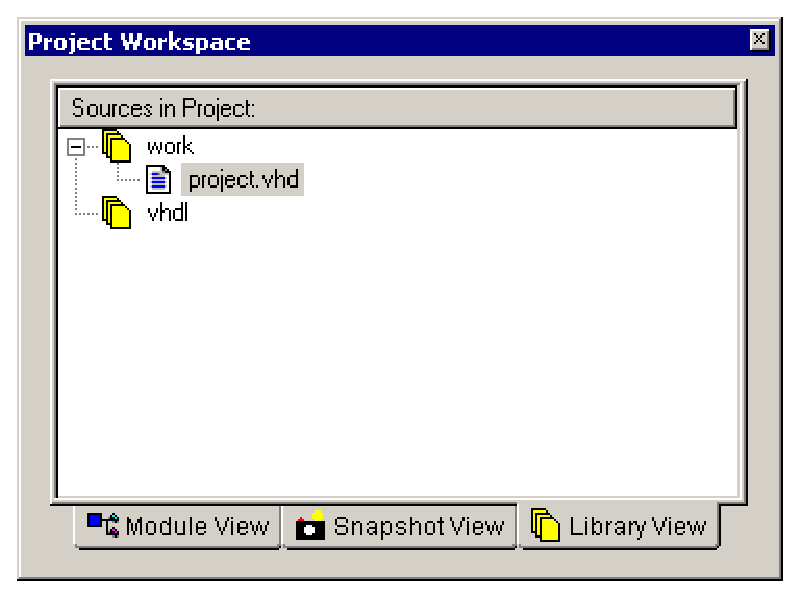
\includegraphics[height=4cm]{ise_1}} \qquad
  \subfigure[Creating the
  library.\label{fig:ise_2}]{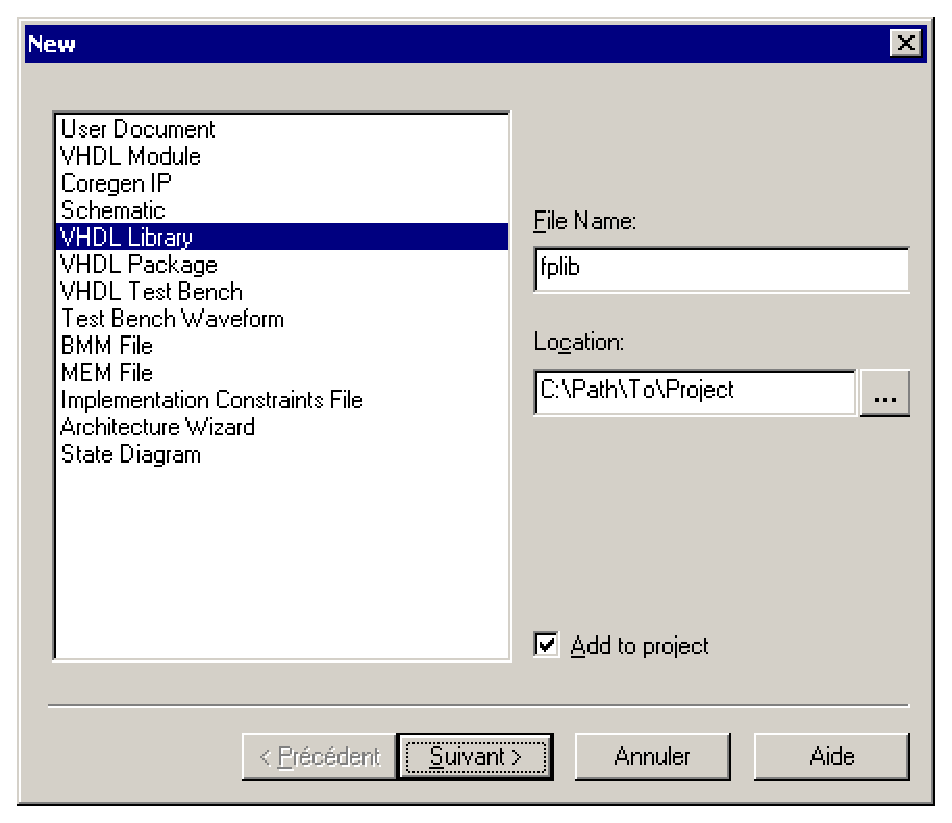
\includegraphics[height=5.5cm]{ise_2}} \\
  \subfigure[Adding source
  files.\label{fig:ise_3}]{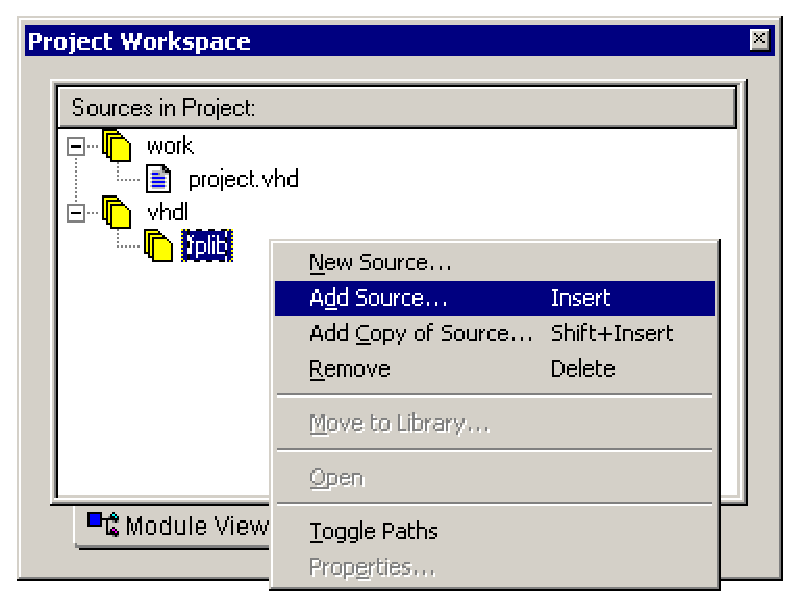
\includegraphics[height=4cm]{ise_3}} \qquad
  \subfigure[FPLibrary is
  loaded.\label{fig:ise_4}]{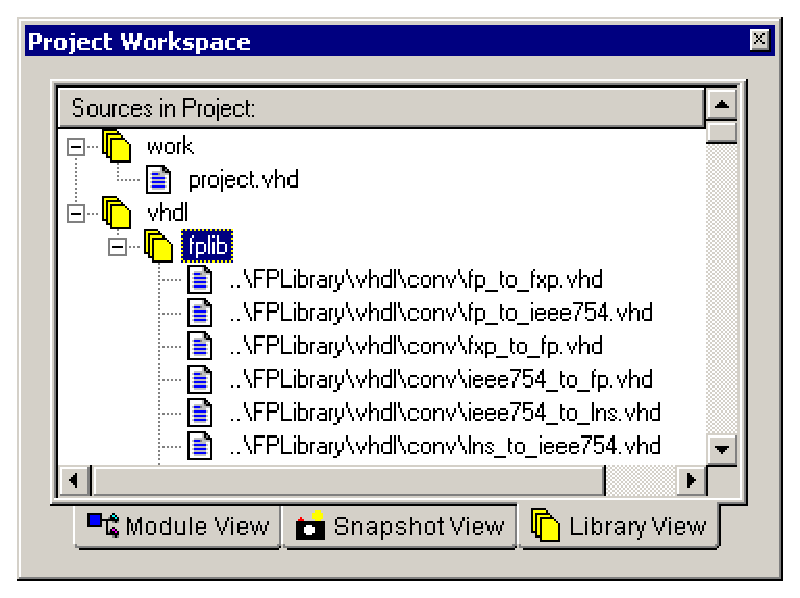
\includegraphics[height=4cm]{ise_4}}
  \caption{Xilinx Project Navigator screenshots.}
\end{figure}

\subsubsection{XST (Xilinx Synthesis Technology)}

This section describes the FPLibrary installation steps for those who
use Xilinx tools in a command-line fashion, and therefore do not want
to create a project using ISE.

To use the library, you just have to use the file
\texttt{FPLibrary-\ver/misc/xst/fplib.prj} and merge it into your own
\texttt{.prj} file.

You can also compile each VHDL source file separatly using a script,
as the order of compilation is given by
\texttt{FPLibrary-\ver/misc/xst/fplib.prj}. Be sure to compile the
FPLibrary files into the \texttt{fplib} library, using the
command-line option \texttt{-work\_lib fplib}.

\subsection{Using FPLibrary operators}

To use FPLibrary operators in your own circuits, just add the
following lines to the source code of the concerned components:\\
\texttt{library fplib;}\\
\texttt{use fplib.pkg\_fplib.all;}

You then just have to instantiate the operators in the usual way. If
FPLibrary was correctly integrated into your project as the
\texttt{fplib} library (as described in Section~\ref{sec:synth}), the
synthesizer will automatically import them.

See Sections~\ref{sec:op} and \ref{sec:conv} for a complete
description of the operators and their interfaces.


\section{Examples}
A few simple examples can be found in the directory\texttt{FPLibrary-\ver/vhdl/test/examples}.



\chapter{Number representation formats}

\section{Floating-point}

The floating-point (FP) number format used in FPLibrary is mainly
inspired from the IEEE-754 standard~\cite{IEEE754}. Its main idea is
to represent numbers with a fixed-point normalized mantissa multiplied
by an order of magnitude (an integer power of $2$). For example: $1.25
\times 2^{21}$, $-1.75 \times 2^{18}$, $1.00 \times 2^{-5}$, ...

This representation is parameterized by two bitwidths $w_E$ and $w_F$.
An FP number $X$ is then represented as a vector of $w_E+w_F+3$ bits,
and can be partitioned in $4$ fields as shown Figure~\ref{fig:fp_fmt}:
\begin{itemize}
\item $\mathrm{exn}$ ($2$ bits): the exception tag;
\item $S_X$ ($1$ bit): the sign bit;
\item $E_X$ ($w_E$ bits): the exponent (biased by $E_0 =
  2^{w_E-1}-1$);
\item $F_X$ ($w_F$ bits): the fraction (mantissa).
\end{itemize}

\begin{figure}[htp!]
  \centering \input{fp_fmt.pstex_t}
\caption{Floating-point number format.}
\label{fig:fp_fmt}
\end{figure}

The value of $X$ is given according to the exception tag:
\begin{itemize}
\item zero ($\mathrm{exn} = 00$): $X = (-1)^{S_X} \times 0$\\
  note that $0$ is signed, as stated in the IEEE-754 standard;
\item normalized number ($\mathrm{exn} = 01$): $X = (-1)^{S_X} \times
  1.F_X \times 2^{E_X-E_0}$;
\item infinity ($\mathrm{exn} = 10$): $X = (-1)^{S_X} \times \infty$;
\item not-a-number ($\mathrm{exn} = 11$): $X = \mathrm{NaN}$\\
  $\mathrm{NaN}$ is an undefined value, such as $0/0$ or $\infty -
  \infty$.
\end{itemize}

\emph{Remark:} FPLibrary does not handle the denormalized numbers
described by the IEEE-754 standard.

\section{Logarithmic number system}

The logarithmic number system (LNS) was first introduced by
Schwartzlander in~\cite{Swartzlander75}. The idea here is to use a
fixed-point exponent instead of a mantissa. For example: $2^{42.25}$,
$2^{-12.50}$, $-2^{23.75}$, ...

In FPLibrary, this representation is also parameterized by $w_E$ and
$w_F$, and an LNS number $X$ is represented as a vector of $w_E+w_F+3$
bits, and can be partitioned in $4$ fields as shown
Figure~\ref{fig:lns_fmt}:
\begin{itemize}
\item $\mathrm{exn}$ ($2$ bits): the exception tag;
\item $S_X$ ($1$ bit): the sign bit;
\item $E_{L_X}$ ($w_E$ bits): the integer part of the logarithm $L_X$;
\item $F_{L_X}$ ($w_F$ bits): the fractional part of the logarithm.
\end{itemize}

\emph{Remark:} the logarithm $L_X = E_{L_X}.F_{L_X}$ is represented in
$2$'s complement.

\begin{figure}[htp!]
  \centering \input{lns_fmt.pstex_t}
\caption{Logarithmic number format.}
\label{fig:lns_fmt}
\end{figure}

As for FP numbers, the exception tag dictates the value of $X$:
\begin{itemize}
\item zero ($\mathrm{exn} = 00$): $X = (-1)^{S_X} \times 0$;
\item general case ($\mathrm{exn} = 01$): $X = (-1)^{S_X} \times
  2^{L_X}$ where $L_X = E_{L_X}.F_{L_X}$;
\item infinity ($\mathrm{exn} = 10$): $X = (-1)^{S_X} \times \infty$;
\item not-a-number ($\mathrm{exn} = 11$): $X = \mathrm{NaN}$.
\end{itemize}

\chapter{Arithmetic operators}
\label{sec:op}

\section{Addition / subtraction}

\subsection{Synopsis}

\begin{small}
\begin{verbatim}
  component Add is
    generic ( fmt : format;
              wE  : positive := 6;
              wF  : positive := 13 );
    port ( nA : in  std_logic_vector(wE+wF+2 downto 0);
           nB : in  std_logic_vector(wE+wF+2 downto 0);
           nR : out std_logic_vector(wE+wF+2 downto 0) );
  end component;

  component Add_Clk is
    generic ( fmt : format;
              wE  : positive := 6;
              wF  : positive := 13;
              reg : boolean  := true );
    port ( nA  : in  std_logic_vector(wE+wF+2 downto 0);
           nB  : in  std_logic_vector(wE+wF+2 downto 0);
           nR  : out std_logic_vector(wE+wF+2 downto 0);
           clk : in  std_logic );
  end component;

  function addLatency( fmt    : format;
                       wE, wF : positive ) return natural;
\end{verbatim}
\end{small}

\subsection{Parameter mapping}

\subsubsection{Generic parameters}

\begin{description}
\item[\ttfamily fmt] The number system for the operands and result.
  Should be set to either \texttt{FP} or \texttt{LNS}.
\item[\ttfamily wE] The value of $w_E$ used in the representation of
  the operands and result (default: \texttt{6}).
\item[\ttfamily wF] The value of $w_F$ used in the representation of
  the operands and result (default: \texttt{13}).
\item[\ttfamily reg] Indicates if the design should be pipelined or
  not (default: \texttt{yes}).
\end{description}

\subsubsection{Signal ports}

\begin{description}
\item[{\ttfamily nA}, {\ttfamily nB}] The two operands $A$ and $B$.
\item[\ttfamily nR] The result $R = A + B$.
\item[\ttfamily clk] The clock signal.
\end{description}

\subsection{Description}

\begin{description}
\item[\ttfamily Add] The pure combinatorial version of the
  addition/subtraction operator.
\item[\ttfamily Add\_Clk] The combinatorial version if \texttt{reg} is
  set to \texttt{no} or the pipelined version if \texttt{reg} is set
  to \texttt{yes}.
\item[\ttfamily addLatency] The number of stages of the pipelined
  version of the operator.
\end{description}

\emph{Remark:} the result is rounded to nearest for FP operators,
but this rounding cannot be achieved in LNS. See \cite{DetDin03} for
more details.

\newpage
\section{Multiplication}

\subsection{Synopsis}

\begin{small}
\begin{verbatim}
  component Mul is
    generic ( fmt : format;
              wE  : positive := 6;
              wF  : positive := 13 );
    port ( nA : in  std_logic_vector(wE+wF+2 downto 0);
           nB : in  std_logic_vector(wE+wF+2 downto 0);
           nR : out std_logic_vector(wE+wF+2 downto 0) );
  end component;

  component Mul_Clk is
    generic ( fmt : format;
              wE  : positive := 6;
              wF  : positive := 13;
              reg : boolean  := true );
    port ( nA  : in  std_logic_vector(wE+wF+2 downto 0);
           nB  : in  std_logic_vector(wE+wF+2 downto 0);
           nR  : out std_logic_vector(wE+wF+2 downto 0);
           clk : in  std_logic );
  end component;

  function mulLatency( fmt    : format;
                       wE, wF : positive ) return natural;
\end{verbatim}
\end{small}

\subsection{Parameter mapping}

\subsubsection{Generic parameters}

\begin{description}
\item[\ttfamily fmt] The number system for the operands and result.
  Should be set to either \texttt{FP} or \texttt{LNS}.
\item[\ttfamily wE] The value of $w_E$ used in the representation of
  the operands and result (default: \texttt{6}).
\item[\ttfamily wF] The value of $w_F$ used in the representation of
  the operands and result (default: \texttt{13}).
\item[\ttfamily reg] Indicates if the design should be pipelined or
  not (default: \texttt{yes}).
\end{description}

\subsubsection{Signal ports}

\begin{description}
\item[{\ttfamily nA}, {\ttfamily nB}] The two operands $A$ and $B$.
\item[\ttfamily nR] The result $R = A \times B$.
\item[\ttfamily clk] The clock signal.
\end{description}

\subsection{Description}

\begin{description}
\item[\ttfamily Mul] The pure combinatorial version of the
  multiplication operator.
\item[\ttfamily Mul\_Clk] The combinatorial version if \texttt{reg} is
  set to \texttt{no} or the pipelined version if \texttt{reg} is set
  to \texttt{yes}.
\item[\ttfamily mulLatency] The number of stages of the pipelined
  version of the operator.
\end{description}

\emph{Remark:} the result is rounded to nearest for both FP and LNS
operators.

\newpage
\section{Division}

\subsection{Synopsis}

\begin{small}
\begin{verbatim}
  component Div is
    generic ( fmt : format;
              wE  : positive := 6;
              wF  : positive := 13 );
    port ( nA : in  std_logic_vector(wE+wF+2 downto 0);
           nB : in  std_logic_vector(wE+wF+2 downto 0);
           nR : out std_logic_vector(wE+wF+2 downto 0) );
  end component;

  component Div_Clk is
    generic ( fmt : format;
              wE  : positive := 6;
              wF  : positive := 13;
              reg : boolean  := true );
    port ( nA  : in  std_logic_vector(wE+wF+2 downto 0);
           nB  : in  std_logic_vector(wE+wF+2 downto 0);
           nR  : out std_logic_vector(wE+wF+2 downto 0);
           clk : in  std_logic );
  end component;

  function divLatency( fmt    : format;
                       wE, wF : positive ) return natural;
\end{verbatim}
\end{small}

\subsection{Parameter mapping}

\subsubsection{Generic parameters}

\begin{description}
\item[\ttfamily fmt] The number system for the operands and result.
  Should be set to either \texttt{FP} or \texttt{LNS}.
\item[\ttfamily wE] The value of $w_E$ used in the representation of
  the operands and result (default: \texttt{6}).
\item[\ttfamily wF] The value of $w_F$ used in the representation of
  the operands and result (default: \texttt{13}).
\item[\ttfamily reg] Indicates if the design should be pipelined or
  not (default: \texttt{yes}).
\end{description}

\subsubsection{Signal ports}

\begin{description}
\item[\ttfamily nA] The dividend $A$.
\item[\ttfamily nB] The divisor $B$.
\item[\ttfamily nR] The result $R = A / B$.
\item[\ttfamily clk] The clock signal.
\end{description}

\subsection{Description}

\begin{description}
\item[\ttfamily Div] The pure combinatorial version of the
  division operator.
\item[\ttfamily Div\_Clk] The combinatorial version if \texttt{reg} is
  set to \texttt{no} or the pipelined version if \texttt{reg} is set
  to \texttt{yes}.
\item[\ttfamily divLatency] The number of stages of the pipelined
  version of the operator.
\end{description}

\emph{Remark:} the result is rounded to nearest for both FP and LNS
operators.

\newpage
\section{Square root}

\subsection{Synopsis}

\begin{small}
\begin{verbatim}
  component Sqrt is
    generic ( fmt : format;
              wE  : positive := 6;
              wF  : positive := 13 );
    port ( nA : in  std_logic_vector(wE+wF+2 downto 0);
           nR : out std_logic_vector(wE+wF+2 downto 0) );
  end component;

  component Sqrt_Clk is
    generic ( fmt : format;
              wE  : positive := 6;
              wF  : positive := 13;
              reg : boolean  := true );
    port ( nA  : in  std_logic_vector(wE+wF+2 downto 0);
           nR  : out std_logic_vector(wE+wF+2 downto 0);
           clk : in  std_logic );
  end component;

  function sqrtLatency( fmt    : format;
                        wE, wF : positive ) return natural;
\end{verbatim}
\end{small}

\subsection{Parameter mapping}

\subsubsection{Generic parameters}

\begin{description}
\item[\ttfamily fmt] The number system for the operand and result.
  Should be set to either \texttt{FP} or \texttt{LNS}.
\item[\ttfamily wE] The value of $w_E$ used in the representation of
  the operand and result (default: \texttt{6}).
\item[\ttfamily wF] The value of $w_F$ used in the representation of
  the operand and result (default: \texttt{13}).
\item[\ttfamily reg] Indicates if the design should be pipelined or
  not (default: \texttt{yes}).
\end{description}

\subsubsection{Signal ports}

\begin{description}
\item[\ttfamily nA] The operand $A$.
\item[\ttfamily nR] The result $R = \sqrt{A}$.
\item[\ttfamily clk] The clock signal.
\end{description}

\subsection{Description}

\begin{description}
\item[\ttfamily Sqrt] The pure combinatorial version of the
  division operator.
\item[\ttfamily Sqrt\_Clk] The combinatorial version if \texttt{reg} is
  set to \texttt{no} or the pipelined version if \texttt{reg} is set
  to \texttt{yes}.
\item[\ttfamily sqrtLatency] The number of stages of the pipelined
  version of the operator.
\end{description}

\emph{Remark:} the result is rounded to nearest for both FP and LNS
operators.

\chapter{Conversion operators}
\label{sec:conv}

\section{Fixed-point/floating-point conversions}
\subsection{Synopsis}

\begin{small}
\begin{verbatim}
  component FXP_To_FP is
    generic ( wE    : positive := 6;
              wF    : positive := 13;
              wFX_I : positive := 6;
              wFX_F : positive := 13 );
    port ( nA : in  std_logic_vector(wFX_I+wFX_F-1 downto 0);
           nR : out std_logic_vector(wE+wF+2 downto 0));
  end component;

  component FP_To_FXP is
    generic ( wE    : positive := 6;
              wF    : positive := 13;
              wFX_I : positive := 6;
              wFX_F : positive := 13 );
    port ( nA : in  std_logic_vector(wE+wF+2 downto 0);
           nR : out std_logic_vector(wFX_I+wFX_F-1 downto 0));
  end component;
\end{verbatim}
\end{small}

\section{Conversion between IEEE754 and FPLibrary floating-point formats}

The IEEE754 format is the standard format used in most PCs.  Single
precision is (wE=8, wF=23), double-precision is (wE=11, wF=52). This
format is more memory-efficient, since it encodes infinities and zeros
respectively as the largest and smallest values of the
exponent. Conversely, the internal FPLibrary format is more
hardware-efficient. It codes these special values as special bits, and
therefore doesn't need to decode and encode special exponent values
into the corresponding bits at each operation.

Therefore, a pipeline of operators should use the FPLibrary
format. Conversion from and to the IEEE754 format should be performed
essentially at input and output. 

Remark: If you store single precision data in internal memory blocks
such as BlockRams or M9K, you will have 36 bits to store a single
precision data, which means that you may keep the single precision
FPLibrary format (8+23+3=34 bits).

\subsection{Synopsis}
\begin{small}
\begin{verbatim}
  component IEEE754_To_FP is
    generic ( wE : positive := 6;
              wF : positive := 13 );
    port ( nA : in  std_logic_vector(wE+wF downto 0);
           nR : out std_logic_vector(wE+wF+2 downto 0));
  end component;

  component FP_To_IEEE754 is
    generic ( wE : positive := 6;
              wF : positive := 13 );
    port ( nA : in  std_logic_vector(wE+wF+2 downto 0);
           nR : out std_logic_vector(wE+wF downto 0));
  end component;
\end{verbatim}
\end{small}
\subsection{Description}



\begin{description}
\item[\ttfamily IEEE754\_To\_FP] Converts the IEE-754 format on  wF+wE+1 bits
  into the internal  FPLibrary format on wF+wE+3 bits.  
\item[\ttfamily FP\_To\_IEEE754] Converts the
   internal  FPLibrary format on wF+wE+3 bits 
   into the  
   IEE-754 format on  wF+wE+1 bits.  
\end{description}

\section{Conversion between IEEE754 and LNS  formats}
\subsection{Synopsis}

\begin{small}
\begin{verbatim}
  component IEEE754_To_LNS is
    generic ( wE : positive := 6;
              wF : positive := 13 );
    port ( nA : in  std_logic_vector(wE+wF downto 0);
           nR : out std_logic_vector(wE+wF+2 downto 0));
  end component;

  component LNS_To_IEEE754 is
    generic ( wE : positive := 6;
              wF : positive := 13 );
    port ( nA : in  std_logic_vector(wE+wF+2 downto 0);
           nR : out std_logic_vector(wE+wF downto 0));
  end component;
end package;
\end{verbatim}
\end{small}





\bibliographystyle{plain}
\begin{thebibliography}{10}
  \addcontentsline{toc}{chapter}{Bibliography}
  
\bibitem{DetDin03} J.~ Detrey and F.~de~Dinechin.  \newblock A {VHDL}
  library of {LNS} operators.  \newblock In {\em 37th Asilomar
    Conference on Signals, Systems and Computers}, Pacific Grove, USA,
  October 2003.
  
\bibitem{IEEE754} {IEEE} standard for binary floating-point
  arithmetic.  \newblock ANSI/IEEE Std 754-1985, 1985.
  
\bibitem{Swartzlander75} E.~E. Swartzlander and G.~Alexopoulos.
  \newblock The sign/logarithm number system.  \newblock {\em IEEE
    Transactions on Computers}, 24(12):1238--1242, December 1975.
\end{thebibliography}

% \appendix

% \chapter{File hierarchy}
% \label{sec:hierarchy}

% \chapter{Example}
% \label{sec:example}

\end{document}
